%me=0 student solutions (ps file), me=1 - my solutions (sol file), me=2 - assignment (hw file)
\def\me{0}
\def\num{1}  %homework number
\def\due{Thursday, March 10}  %due date
\def\course{DS-GA.1008 Deep Learning} %course name, changed only once
\def\name{R2DEEP2 (Ankit Vani, Srivas Venkatesh)}   %student changes (instructor keeps!)
%
\iffalse
INSTRUCTIONS: replace # by the homework number.
(if this is not ps#.tex, use the right file name)

  Clip out the ********* INSERT HERE ********* bits below and insert
appropriate TeX code.  Once you are done with your file, run

  ``latex ps#.tex''

from a UNIX prompt.  If your LaTeX code is clean, the latex will exit
back to a prompt.  To see intermediate results, type

  ``xdvi ps#.dvi'' (from UNIX prompt)
  ``yap ps#.dvi'' (if using MikTex in Windows)

after compilation. Once you are done, run

  ``dvips ps#.dvi''

which should print your file to the nearest printer.  There will be
residual files called ps#.log, ps#.aux, and ps#.dvi.  All these can be
deleted, but do not delete ps1.tex. To generate postscript file ps#.ps,
run

  ``dvips -o ps#.ps ps#.dvi''

I assume you know how to print .ps files (``lpr -Pprinter ps#.ps'')
\fi
%
\title{Deep Learning}
\documentclass[11pt]{article}
\usepackage{amsfonts,amsmath,physics}
\usepackage[backend=bibtex,sorting=none]{biblatex}
\usepackage{latexsym, graphicx}
\usepackage{amssymb, gensymb}
\usepackage{mathtools}
\usepackage{clrscode3e}
\usepackage{longtable}
\usepackage{tikz}
\usepackage{bm}
\usepackage{hyperref}
\usetikzlibrary{trees}
\usepackage{tikz-qtree}
\usepackage{graphicx,float,subfig}
\setlength{\oddsidemargin}{.0in}
\setlength{\evensidemargin}{.0in}
\setlength{\textwidth}{6.5in}
\setlength{\topmargin}{-0.4in}
\setlength{\textheight}{8.5in}

\addbibresource{bibliography.bib}
\graphicspath{ {../images/} }

\newcommand{\handout}[5]{
   \renewcommand{\thepage}{#1, Page \arabic{page}}
   \noindent
   \begin{center}
   \framebox{
      \vbox{
    \hbox to 5.78in { {\bf \course} \hfill #2 }
       \vspace{4mm}
       \hbox to 5.78in { {\Large \hfill #5  \hfill} }
       \vspace{2mm}
       \hbox to 5.78in { {\it #3 \hfill #4} }
      }
   }
   \end{center}
   \vspace*{4mm}
}

\newcommand{\LCA}{\mbox{\sf LCA}}

\newcommand{\rs}{\rightsquigarrow}
\newcommand{\ls}{\leftsquigarrow}

\newcounter{pppp}
\newcommand{\prob}{\arabic{pppp}}  %problem number
\newcommand{\increase}{\addtocounter{pppp}{1}}  %problem number

%first argument desription, second number of points
\newcommand{\newproblem}[1]{
\ifnum\me=0
\ifnum\prob>0 \newpage \fi
\increase
\setcounter{page}{1}
\handout{\name, Assignment \num, Section \arabic{pppp}}{\today}{Team: \name}{Due:
\due}{Solutions to Assignment \num}
\section*{Problem \prob~ - #1 \hfill}
\else
\increase
\section*{Problem \num-\prob~ - #1 \hfill}
\fi
}

%\newcommand{\newproblem}[2]{\increase
%\section*{Problem \num-\prob~(#1) \hfill {#2}}
%}

\def\squarebox#1{\hbox to #1{\hfill\vbox to #1{\vfill}}}
\def\qed{\hspace*{\fill}
        \vbox{\hrule\hbox{\vrule\squarebox{.667em}\vrule}\hrule}}
\newenvironment{solution}{\begin{trivlist}\item[]{\bf Solution:}}
                      {\qed \end{trivlist}}
\newenvironment{solsketch}{\begin{trivlist}\item[]{\bf Solution Sketch:}}
                      {\qed \end{trivlist}}
\newenvironment{code}{\begin{tabbing}
12345\=12345\=12345\=12345\=12345\=12345\=12345\=12345\= \kill }
{\end{tabbing}}

%%%%%\newcommand{\eqref}[1]{Equation~(\ref{eq:#1})}

\newcommand{\hint}[1]{({\bf Hint}: {#1})}
%Put more macros here, as needed.
\newcommand{\room}{\medskip\ni}
\newcommand{\brak}[1]{\langle #1 \rangle}
\newcommand{\bit}[1]{\{0,1\}^{#1}}
\newcommand{\zo}{\{0,1\}}
\newcommand{\C}{{\cal C}}

\newcommand{\nin}{\not\in}
\newcommand{\set}[1]{\{#1\}}
\renewcommand{\ni}{\noindent}
\renewcommand{\gets}{\leftarrow}
\renewcommand{\to}{\rightarrow}
\newcommand{\assign}{:=}
\newcommand{\cT}{\mathcal{T}}

\DeclareMathOperator*{\E}{E}
\DeclareMathOperator*{\argmin}{arg\,min}
\DeclareMathOperator*{\argmax}{arg\,max}
\DeclareMathOperator*{\ORA}{\vee}
\newcommand{\R}{\mathbb{R}}

%\DeclarePairedDelimiter{\abs}{\lvert}{\rvert}
%\DeclarePairedDelimiter{\norm}{\lVert}{\rVert}
\DeclarePairedDelimiter{\inprod}{\langle}{\rangle}

\newcommand\Perm[2][n]{\prescript{#1\mkern-2.5mu}{}P_{#2}}

\newcommand{\AND}{\wedge}
\newcommand{\OR}{\vee}

\newcommand{\mexp}{\mathrm{e}}

\makeatletter
\newtoks\@tabtoks
\newcommand\addtabtoks[1]{\global\@tabtoks\expandafter{\the\@tabtoks#1}}
\newcommand\eaddtabtoks[1]{\edef\mytmp{#1}\expandafter\addtabtoks\expandafter{\mytmp}}
\newcommand*\resettabtoks{\global\@tabtoks{}}
\newcommand*\printtabtoks{\the\@tabtoks}
\makeatother

\allowdisplaybreaks


\begin{document}


\newproblem{More Backpropagation}


\begin{enumerate}

\item[1.1] \textbf{Backpropagation through a DAG of modules}
\ifnum\me<2
\begin{solution}\\
Let $o_{max}$ be the output of the \texttt{max} module, and $o_{min}$ be the output of the \texttt{min} module.

Let $i_1$ be the output of the first \texttt{sigmoid} module, and $i_2$ be the output of the second \texttt{sigmoid} module. Furthermore, let $i = \begin{bmatrix} i_1 \\ i_2 \end{bmatrix}$.

We have:
\begin{align*}
\frac{\partial o_{max}}{\partial x_1} &= \frac{\partial o_{max}}{\partial i} \frac{\partial i}{\partial x_1}\\
&= \begin{bmatrix} \frac{\partial o_{max}}{\partial i_1} & \frac{\partial o_{max}}{\partial i_2} \end{bmatrix} \begin{bmatrix} \frac{\partial i_1}{\partial x_1} \\ \frac{\partial i_2}{\partial x_1} \end{bmatrix}\\
&= \begin{bmatrix} 1_{i_1 \geq i_2} & 1_{i_1 < i_2} \end{bmatrix} \begin{bmatrix} \frac{\partial i_1}{\partial x_1} \\ \frac{\partial i_2}{\partial x_1} \end{bmatrix}\\
&= \left(\frac{\partial i_1}{\partial x_1}\right)_{i_1 \geq i_2} + \left(\frac{\partial i_2}{\partial x_1}\right)_{i_1 < i_2}
\end{align*}

Similarly, we have:
\begin{align*}
\frac{\partial o_{min}}{\partial x_1} &= \frac{\partial o_{min}}{\partial i} \frac{\partial i}{\partial x_1}\\
&= \begin{bmatrix} \frac{\partial o_{min}}{\partial i_1} & \frac{\partial o_{min}}{\partial i_2} \end{bmatrix} \begin{bmatrix} \frac{\partial i_1}{\partial x_1} \\ \frac{\partial i_2}{\partial x_1} \end{bmatrix}\\
&= \begin{bmatrix} 1_{i_1 < i_2} & 1_{i_1 \geq i_2} \end{bmatrix} \begin{bmatrix} \frac{\partial i_1}{\partial x_1} \\ \frac{\partial i_2}{\partial x_1} \end{bmatrix}\\
&= \left(\frac{\partial i_1}{\partial x_1}\right)_{i_1 < i_2} + \left(\frac{\partial i_2}{\partial x_1}\right)_{i_1 \geq i_2}
\end{align*}

Finally, we have:
\begin{align*}
\frac{\partial E}{\partial x_1} &= \frac{\partial E}{\partial y} \frac{\partial (o_{max} + o_{min})}{\partial x_1}\\
&= \frac{\partial E}{\partial y} \left( \frac{\partial o_{max}}{\partial x_1} + \frac{\partial o_{min}}{\partial x_1} \right)\\
&= \frac{\partial E}{\partial y} \left( \left(\frac{\partial i_1}{\partial x_1}\right)_{i_1 \geq i_2} + \left(\frac{\partial i_2}{\partial x_1}\right)_{i_1 < i_2} + \left(\frac{\partial i_1}{\partial x_1}\right)_{i_1 < i_2} + \left(\frac{\partial i_2}{\partial x_1}\right)_{i_1 \geq i_2} \right)\\
&= \frac{\partial E}{\partial y} \left( \frac{\partial i_1}{\partial x_1} + \frac{\partial i_2}{\partial x_1} \right) \tag{Only one of $i_1 \geq i_2$ or $i_1 < i_2$ can be true}\\
&= \frac{\partial E}{\partial y} \frac{\partial i_1}{\partial x_1} \tag{$i_2$ does not depend on $x_1$}\\
&= \frac{\partial E}{\partial y} \cdot \frac{\partial}{\partial x_1} \frac{1}{1+e^{-x_1}}\\
&= \frac{\partial E}{\partial y} \frac{e^{-x_1}}{(1+e^{-x_1})^2}\\
&= \frac{\partial E}{\partial y} \frac{e^{x_1}}{(e^{x_1}+1)^2}\\
\end{align*}

From the network structure, we can see that the partial derivatives of $o_{max}$ and $o_{min}$ and with respect to $x_2$ would be the same as that with respect to $x_1$, since all the dependencies are similar beyond that layer.

Thus, we have:
\begin{align*}
\frac{\partial o_{max}}{\partial x_2} &= \left(\frac{\partial i_1}{\partial x_2}\right)_{i_1 \geq i_2} + \left(\frac{\partial i_2}{\partial x_2}\right)_{i_1 < i_2}\\
\frac{\partial o_{min}}{\partial x_2} &= \left(\frac{\partial i_1}{\partial x_2}\right)_{i_1 < i_2} + \left(\frac{\partial i_2}{\partial x_2}\right)_{i_1 \geq i_2}
\end{align*}

And similar to above, we get:
\begin{align*}
\frac{\partial E}{\partial x_2} &= \frac{\partial E}{\partial y} \left( \left(\frac{\partial i_1}{\partial x_2}\right)_{i_1 \geq i_2} + \left(\frac{\partial i_2}{\partial x_2}\right)_{i_1 < i_2} + \left(\frac{\partial i_1}{\partial x_2}\right)_{i_1 < i_2} + \left(\frac{\partial i_2}{\partial x_2}\right)_{i_1 \geq i_2} \right)\\
&= \frac{\partial E}{\partial y} \left( \frac{\partial i_1}{\partial x_2} + \frac{\partial i_2}{\partial x_2} \right) \tag{Only one of $i_1 \geq i_2$ or $i_1 < i_2$ can be true}\\
&= \frac{\partial E}{\partial y} \frac{e^{x_2}}{(e^{x_2}+1)^2}
\end{align*}

\end{solution}
\fi


\item[1.2] \textbf{Batch Normalization}
\begin{enumerate}
\item[1.2.1] Given $\frac{\partial E}{\partial y_k}$ write down $\frac{\partial E}{\partial x_k}$, where E is the energy function.
\ifnum\me<2
\begin{solution}
\\For this problem we are going to consider the notation used in the paper \cite{BN} as the question is ill-formed.
That is, we are given the function 
\begin{align*}
y^{(k)} &= \frac{x^{(k)} - E(x^{(k)})}{\sqrt{(\sigma(x^{(k)}))^2}}
\end{align*}
where $k$ is a dimension of the $d$ dimensional input and we take these mean and variance along the batch inputs on those dimensions. Now assuming the mini-batch size to be $m$, that is we have $m$ samples, we get the following along a particular dimension:
\begin{align*}
y_i &= \frac{x_i-E(x)}{\sqrt{(\sigma(x))^2}}
\end{align*}
where $i$ ranges from $1 \ldots m$. This is the same across all the dimensions and the normalization of each dimension is independent of the other. Then we can write the gradient of the energy function wrt. $x^{(k)}_i$ as follows:
\begin{equation}
\frac{\partial E}{\partial x^{(k)}_i} = \sum_{j=1}^m \frac{\partial E}{\partial y^{(k)}_j} \cdot \frac{\partial y^{(k)}_j}{\partial x^{(k)}_i}
\label{eq1}
\end{equation}
Dropping the superscripts for convenience (we will later get it back by showing it as vector elements), we see the following:
\begin{equation}
\frac{\partial y_j}{\partial x_i} =
\begin{cases}
-\frac{1}{m\sigma(x)} - \frac{(x_j-E(x)) (x_i-E(x))}{m\sigma(x)^3} & \text{if } j \neq i\\
(1-\frac{1}{m})\cdot \frac{1}{\sigma(x)} - \frac{(x_i-E(x))^2}{m\sigma(x)^3} & \text{if } j = i
\end{cases}
\label{eq2}
\end{equation}
The above is arrived at by differentiation by parts and using the fact that $(\sigma(x))^2 = E(x^2) - E(x)^2$. Putting back the superscripts we get:
\begin{equation}
\frac{\partial E}{\partial x^{(k)}} =
\begin{bmatrix}
\frac{\partial E}{\partial x^{(k)}_1} & \frac{\partial E}{\partial x^{(k)}_2} & \cdots & \frac{\partial E}{\partial x^{(k)}_m}
\end{bmatrix}
\label{eq3}
\end{equation}
Substituting results from (\ref{eq1}),(\ref{eq2}) in (\ref{eq3}), we get what the question asks.
\end{solution}
\fi

\item[1.2.2] Can you derive
a way to incorporate a learnable shift variable into the current formula? Let’s assume
the considered variable is denoted by $\epsilon$. Please write down the forward and backward
pass, and derive $\frac{\partial E}{\partial \epsilon}$

\ifnum\me<2
\begin{solution}
\\We can do this by changing the batch normalization function as follows:
$$y^{(k)} = \frac{x^{(k)} - E(x^{(k)})}{\sqrt{(\sigma(x^{(k)}))^2}} + \epsilon^{(k)}$$
That is we introduce a learnable shift to our normalization. With that the gradient is simply computed as:
$$\frac{\partial E}{\partial \epsilon^{(k)}} =
\begin{bmatrix}
\frac{\partial E}{\partial y^{(k)}_1} & \frac{\partial E}{\partial y^{(k)}_2} & \cdots & \frac{\partial E}{\partial y^{(k)}_m}
\end{bmatrix}
\cdot
\begin{bmatrix}
1 \\ 1 \\ \cdots \\ 1
\end{bmatrix}
= \sum_{i=1}^{m} \frac{\partial E}{\partial y^{(k)}_i}
$$
Thus we can write the required gradient in the form
$$\frac{\partial E}{\partial \epsilon} =
\begin{bmatrix}
\sum_{i=1}^{m} \frac{\partial E}{\partial y^{(1)}_i}\\
\sum_{i=1}^{m} \frac{\partial E}{\partial y^{(2)}_i}\\
\cdots\\
\sum_{i=1}^{m} \frac{\partial E}{\partial y^{(d)}_i}
\end{bmatrix}$$
\end{solution}
\fi
\end{enumerate}
\end{enumerate}

\newproblem{STL-10: semi-supervised image recognition}
\ifnum\me<2
\begin{solution}
\\We performed our experiments on the STL-10 dataset \cite{coates2011analysis} to classify real world images into 10 classes: airplane, bird, car, cat, deer, dog, horse, monkey, ship, truck.
\\Since STL-10 is a dataset with a much larger corpus of unlabeled data, we used ideas from \cite{conv_kmeans} to pre-train first 4 layers of our network using the unsupervised data. We also use various augmentations and a multi-scale architecture to generalize better. More details are presented below:
\begin{enumerate}
\item \textbf{Overview of the network}
\begin{itemize}
\item \textbf{Dataset, partitioning and pre-processing:}
\\STL-10 dataset has 10 classes with 500 training images per class and 800 test images per class. We had a set of 100 images per class split off from the training images which was used for validation. We thus had 4000 training images, 1000 validation images and 8000 testing images. Besides these labeled data we also have 100,000 unlabeled samples.
\\The loaded training data is converted to YUV colorspace. Spatial contrast normalization is applied to Y component of each image and global normalization to have zero mean and unit variance is performed on the U,V channels. The parameters
used for this normalization are stored and used to normalize the validation and test set as well.
\\The images are converted back to RGB before being passed through our model as the pretraining (which is described later) is done using RGB images.

\item \textbf{Model:}
We use a deep convolutional neural network that takes as input a 96x96 image, produces three scalings of sizes 96x96, 64x64 and 32x32, and passes them through three parallel sets of convolutional layers, with the first few layers pre-learnt through convolutional clustering. The outputs of the three subnetworks are gathered as probability distributions over the output classes, and a weighted average (with learnt weights per class) is taken to produce the overall output of the network through a final logsoftmax operation. We use the negative log-likelihood criterion to compute the classification loss for our network. The model is illustrated in Figure~\ref{fig:model}.\\
We make use of dropout at various stages as described in the figure for regularization. We also make use of Batch Normalization to reduce the effect of internal covariate shift as described in \cite{BN}. This also helps in further regularization, faster training times and helps in appropriately scaling and shifting the feature maps produced by the pre-trained layers. This is important since the layers are not learnt by the classifier but instead clustered independently of it.

\begin{figure}[H]
\label{fig:model}
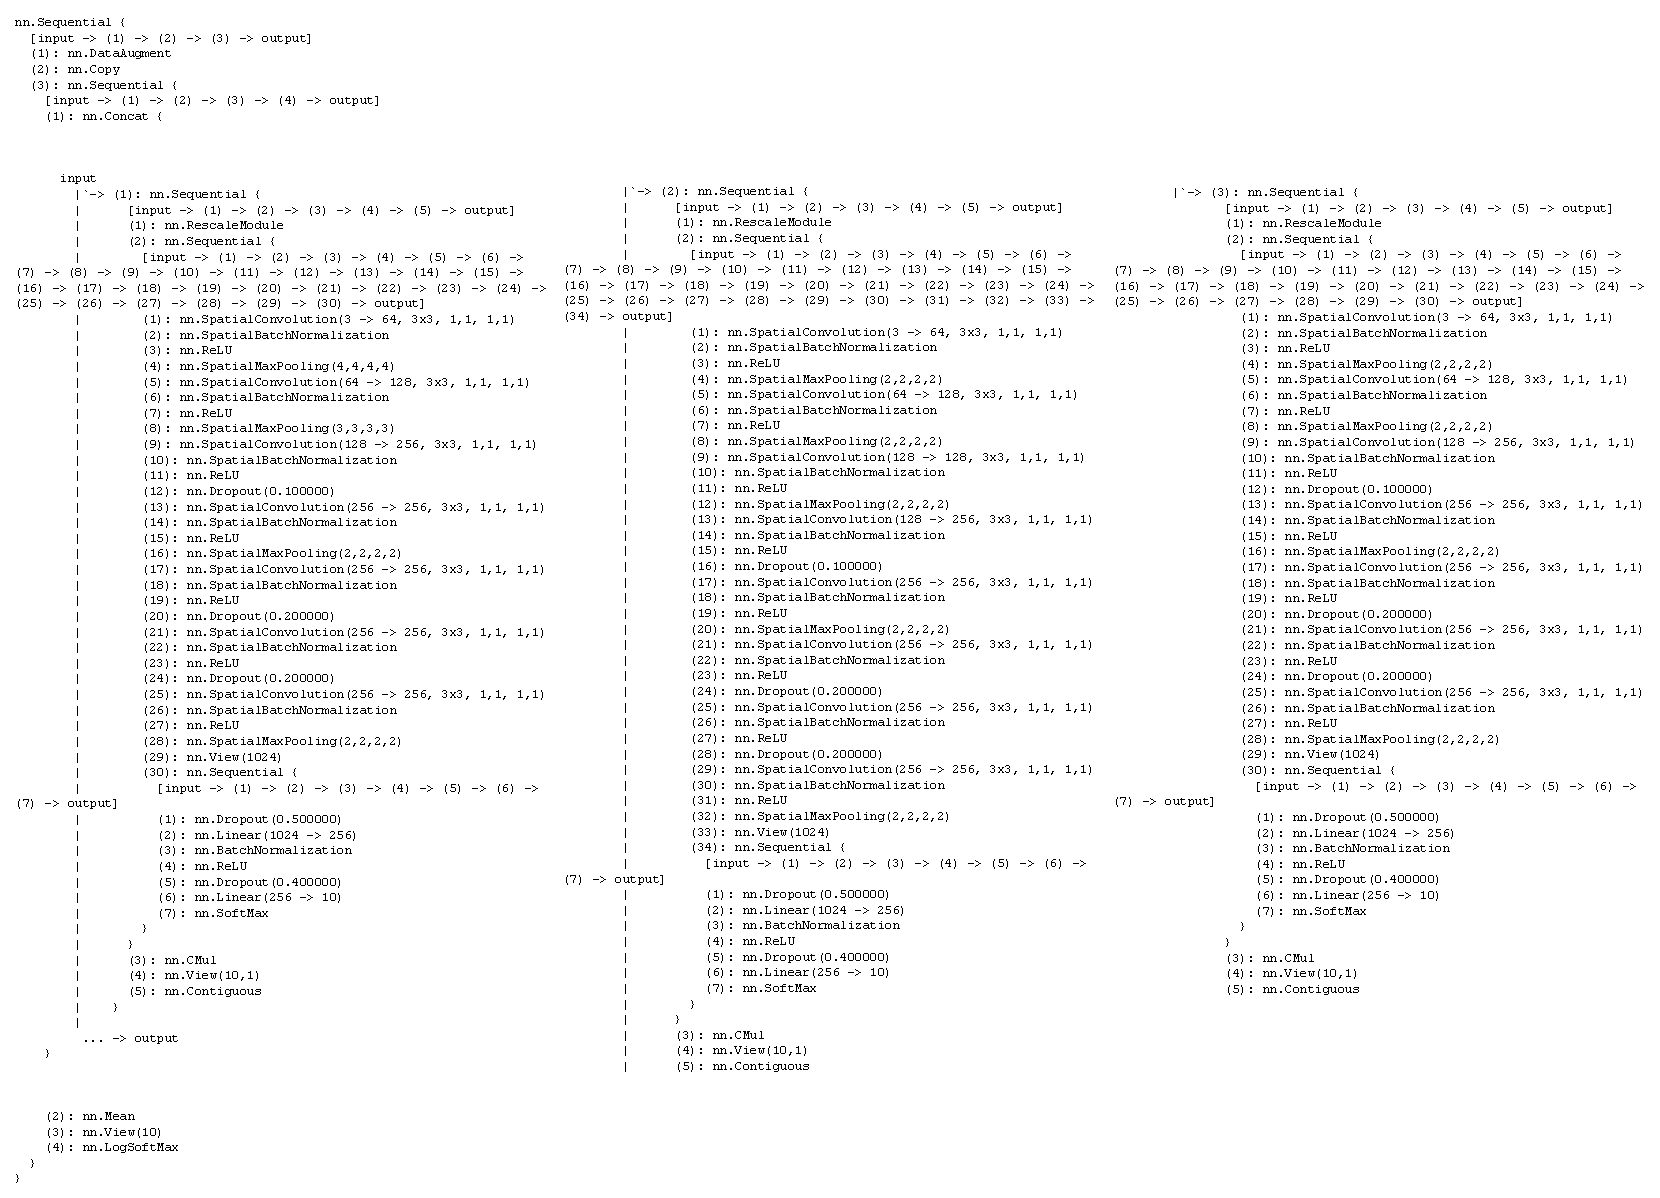
\includegraphics[scale=0.6]{network}
\caption{Our model architecture.}
\end{figure}

\item \textbf{Using the unlabeled data:}
We applied convolutional clustering (\cite{conv_kmeans}) to pre-train the first four layers of the 96x96 subnetwork of our model. For this clustering strategy, we use k-means to cluster patches of images in a 3x3 image space. Since we use 3x3 convolutional filters in our model, we extract random windows of 6x6 from the unlabeled data, and take all the 3x3 patches of this window in a sliding window fashion for clustering. The 3x3 patch that most correlates to one of the centroids is taken as a representative of that window. By performing such a convolutional clustering, we avoid redundant centroids that are just shifted versions of each other.\\
To cluster higher levels of the network, we fix the previous prelearnt levels and pass the unlabeled data as input, and collect the feature maps produced at the level we want to pre-train. We then do convolutional clustering on these feature maps to find the centroids to use as pre-trained convolutional filters in the network.

\item \textbf{Augmentations:}
We perform various data augmentations in order to generalize the network to learn important features invariant of the object classes. These augmentations have been tried and tested in works such as \cite{exemplar} \cite{baidu}. The various augmentations we perform are:
\begin{enumerate}
\item Translation: Vertical and horizontal translation by -15 to +15 pixels.
\item Scaling, Stretching: Scaling height and width independently by 0.75 to 1.25 times.
\item Rotation: Rotation of the image by an angle of -18 to 18 degrees.
\item Contrast Shifting: raise saturation and value (S and V components of the HSV color representation)
of all pixels to a power between 0.25 and 2 (same for all pixels within a patch), multiply
these values by a factor between 0.7 and 1.4, add to them a value between −0.1 and 0.1 as done in \cite{exemplar}
\item Color Shifting: Altering R,G,B channels independently by -30 to +30 as done in \cite{baidu}
\end{enumerate}
We also fill the black spaces created by these transforms (if any) by the mean color at the edges to avoid abrupt color transition. Some of these random transformations applied to a single image are shown below (the combined random transform is applied 50 times to possibly see all the above transforms).
\begin{figure}[H]
\centering
\foreach \x in {1,...,51}
{
	\includegraphics[scale=0.2]{lizard\x.png}
	\ifnum\x=17
	\\
	\fi
	\ifnum\x=34
	\\
	\fi
}
\\
\caption{Random transforms applied 50 times to this image to view all possible transforms. First image is the original image.}
\end{figure}


\end{itemize}

\item \textbf{Visualizations:}
\\We try to visualize some of the layers and activations to see how our network has trained. Some of them are shown below:
\begin{itemize}
\item \textbf{First layer filters learnt through clustering:}
\\The 3x3 filers learnt for the first layer by clustering on unlabeled data is shown below.
\begin{figure}[H]
\centering
\foreach \x in {1,...,64}
{
	\includegraphics[scale=0.5]{filter\x.png}
	\ifnum\x=16
	\\
	\fi
	\ifnum\x=32
	\\
	\fi
	\ifnum\x=48
	\\
	\fi
}
\\
\caption{Filters created by clustering on unsupervised data. These are actually 3x3 filters which are enlarged and enhanced for better display}
\end{figure}
The above filters are actually 3x3 in size but are enlarged and enhanced for better display. This might cause it to look a little saturated and diffused at places than what it actually was. As we can see form this figure the learned filters are detecting some prominent edges just as we had expected. Another point to note is that since we are doing convolutional K-means clustering as described in \cite{conv_kmeans} we have avoided generating similar (shifted) filters.

\item \textbf{t-SNE:}
\\We used t-SNE \cite{tsne} to cluster the representation learnt by our network on the second last layer. It did cluster quite well with meaningful groups and neighbours indicating that the representations learnt by our network are quite well in line with the expected classes. Figure (\ref{tsne}) shows images mapped onto their t-SNE points. We see quite well defined behaviour, the classes are mostly grouped distinctly with little confusion between classes such as dogs and cats, planes and birds, horses and deer etc. Although it may be hard to notice such small details in this zoomed out image, upon zooming in you can see clusters of the following in clockwise order from the bottom: airplanes, ships, trucks, cars, horses, deer, birds, monkeys, dogs, cats. We can also see that the non-living objects on the left are separated from the living objects on the right which is quite interesting. Some of these patches are zoomed and displayed in Fig (\ref{patches}).
\begin{figure}[H]
\centering
\includegraphics[keepaspectratio,width=0.6\paperwidth]{tsne_256.png}
\caption{Images displayed on t-SNE clusters of their representations}
\label{tsne}
\end{figure}

\begin{figure}[H]
\subfloat[][Airplanes]{
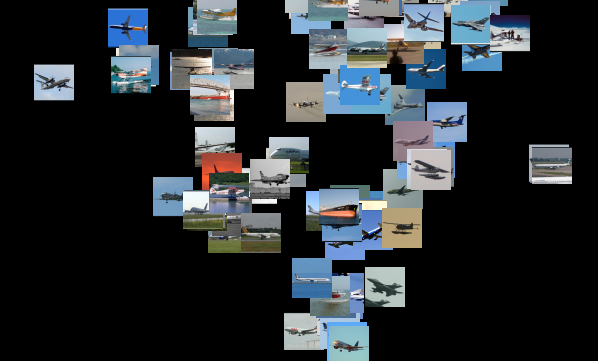
\includegraphics[scale=0.3]{airplanes.png}
}
\subfloat[][Ships]{
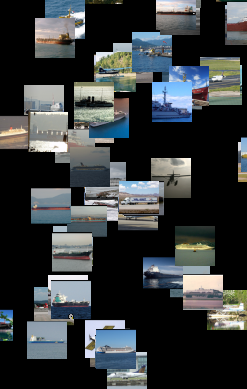
\includegraphics[scale=0.3]{ships.png}
}
\subfloat[][Trucks]{
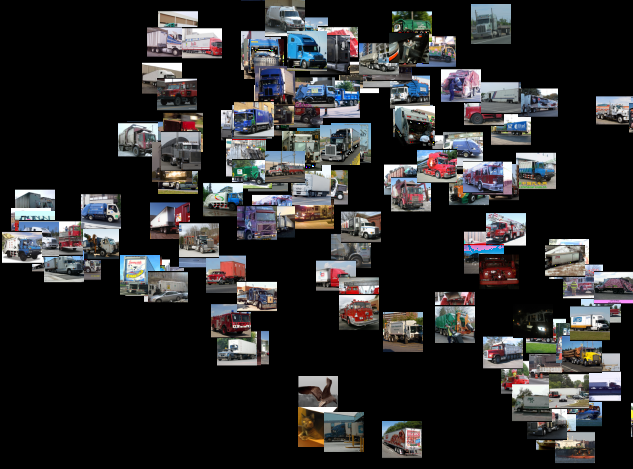
\includegraphics[scale=0.3]{trucks.png}
}
\caption{Some zoomed patches from t-SNE}
\label{patches}
\end{figure}
\end{itemize}
\item \textbf{Experiments and Observations:}
\\We tried experimenting with various architectures, regularizations etc. while trying to make the best use of unsupervised data. In our efforts to strike a balance between accuracy, speed, memory, complexity, generality etc. we decided to go for the model described above.
\\We started with the 2 layer convolutional kmeans filers model described in \cite{conv_kmeans} and saw how such a simple model could utilize the filters learnt from unlabled data to make good predictions. However we noticed that although it was performing well for such a simple network, a more complex network could do better with supervised data alone and hence we decided to go with a complex network making use of the unlabeled data by pre-training them using the convolutional K-means algorithm.
\\We also experimented with larger convolution windows, pooling etc. Finally we also introduced data augmentations to generalize the model. Some of the results of our experiments are shown below.
\begin{table}[h]
\centering
\begin{tabular}{| l | l |}
\hline
\textbf{Network} & \textbf{Accuracy} \\ \hline
2 Layer convolution net as described in \cite{conv_kmeans} & 0.682 \\ \hline
Deep network similar to a single level of our final model in supervised fashion (s) & 0.711 \\ \hline
(s) + initial layers pre-trained and run unsupervised & 0.729 \\ \hline
(s) + initial layers pre-trained and let train in semi supervised fashion (ss) & 0.732 \\ \hline
(ss) + Data Augmentation (sda) & 0.745 \\ \hline
(sda) + multi-scale architecture & 0.754 \\ \hline
\end{tabular}
\caption{Validation accuracies with different network structures.}
\label{table:acc}
\end{table}

\item \textbf{Results:}
\\Using the pre-training obtained from the 100,000 unlabeled data, our model was able to train on the training set of 4000 images and was validated on the test set of size of 8000 images to obtain a test accuracy of 75.2\%. This is the model we submitted to Kaggle.
\end{enumerate}
\end{solution}
\fi


\printbibliography
\end{document}